\documentclass[answers]{submit}
\homework

%TODO: Hier Gruppennummer, Namen, sowie Matrikelnummern einfügen.
\exercisegroup{27}{Eli Kogan-Wang (7251030) \\David Noah Stamm (7249709) \\ Bogdan Rerich (7248483) \\Jan Schreiber(7253698)}

% Folgendes braucht nicht geändert werden
\exercisetl{Universität Paderborn \\ Prof. Dr. Johannes Blömer}
\exerciselecture{Berechenbarkeit und Komplexität -- WS 2022/2023}
\exercisenumber{3}
\exercisehandin{07. November 2022 -- 13:00 Uhr}

%% Generic %%
\newcommand{\Q}{\mathbb{Q}}
\newcommand{\N}{\mathbb{N}}
\newcommand{\C}{\mathbb{C}}
\newcommand{\Z}{\mathbb{Z}}
\newcommand{\R}{\mathbb{R}}
\newcommand{\cO}{\mathcal{O}}
\newcommand{\abs}[1]{\left\vert #1 \right\vert}
\newcommand{\norm}[1]{\left\Vert #1 \right\Vert}
\DeclareMathOperator*{\argmax}{arg\,max}
\DeclareMathOperator*{\argmin}{arg\,min}

\newcommand{\la}{\lambda}
\newcommand{\p}{{\textup P}}
\newcommand{\np}{{\textup NP}}
\newcommand{\cst}{{\tt{cost}}}
\newcommand{\val}{{\tt{value}}}


%% PSEUDOCODE %%%%

\newenvironment{pseudocode}[1]%
{\vspace*{-0.5\baselineskip} \upshape \begin{tabbing}
    99 \= bla \= bla \= bla \= bla \= bla \= bla \= bla \= bla \kill
    #1 \+ \\}%
    {\end{tabbing}}
\newcommand{\keyword}[1]{\texttt{#1}}
\newcommand{\IF}{\keyword{IF} }
\newcommand{\THEN}{\keyword{THEN} \+ \\}
\newcommand{\ELSE}{\< \keyword{ELSE} \\}
\newcommand{\END}{\< \keyword{END} \- \\ }
\newcommand{\OR}{\keyword{OR} }
\newcommand{\AND}{\keyword{AND} }
\newcommand{\RETURN}{\keyword{RETURN} }
\newcommand{\FOR}{\keyword{FOR} }
\newcommand{\WHILE}{\keyword{WHILE} }
\newcommand{\TO}{\keyword{TO} }
\newcommand{\DO}{\keyword{DO} \+ \\ }
\newcommand{\REPEAT}{\keyword{REPEAT} \+ \\ }
\newcommand{\UNTIL}{\< \keyword{UNTIL} \- }


\newcommand{\bestl}{{\tt Beste-L"osung}}
\newcommand{\lb}{{\tt untere-Schranke}}
\newcommand{\mcut}{{\textsc{MaxCut}}}
\newcommand{\opt}{{\textup opt}}
\newcommand{\dt}{{\textup{DTIME}}}
\newcommand{\sat}{{\textup{SAT}}}
\newcommand{\satd}{{\textup{3SAT}}}
\newcommand{\satz}{{\textup{2SAT}}}
\newcommand{\clique}{{\textup{Clique}}}
\newcommand{\ggt}{{\textrm{ggT}}}
\newcommand{\ol}{\overline}
\newcommand{\tm}{{\textrm T}_M}
\newcommand{\msb}{\textrm{MSB}}
\newcommand{\rsopt}{\textrm{RS}_{\textup opt}}
\newcommand{\rsent}{\textrm{RS}_{\textup ent}}
\newcommand{\rsval}{\textrm{RS}_{\textup val}}
\newcommand{\tspopt}{\textrm{TSP}_{\textup opt}}
\newcommand{\tspent}{\textrm{TSP}_{\textup ent}}
\newcommand{\etspent}{\textrm{ETSP}_{\textup ent}}

\newcommand{\tspval}{\textrm{TSP}_{\textup val}}
\newcommand{\etsp}{\textrm{ETSP}}
\newcommand{\nt}{{\textup{NTIME}}}
\newcommand{\tn}{{\textrm{T}_N}}
\newcommand{\ein}{{\textrm{Eintrag}}}
\newcommand{\phis}{\phi_{\textup Start}}
\newcommand{\phia}{\phi_{\textup{accept}}}
\newcommand{\phie}{\phi_{\textup Eintrag}}
\newcommand{\phim}{\phi_{\textup move}}
\newcommand{\susu}{{\textup SubsetSum}}
\newcommand{\ghkreis}{{\textup gH-Kreis}}
\newcommand{\uhkreis}{{\textup uH-Kreis}}
\newcommand{\eue}{{\textup Exakte-"Uberdeckung}}
\newcommand{\kue}{{\textrm{Knoten"uberdeckung}}}
\newcommand{\clopt}{{\textup Clique}_{\textup opt}}
\newcommand{\unabopt}{{\textup Unabh"angig}_{\textup opt}}
\newcommand{\zq}{\Z_q}
\newcommand{\god}{\textrm{G"odel}}
\newcommand{\mr}{M^{\textrm{reject}}}
\newcommand{\diag}{\textrm{Diag}}
\newcommand{\exo}{\textrm{XOR}}
\newcommand{\use}{\textrm{Useful}}
\newcommand{\pot}{{\cal P}(Q)}

\newcommand{\remu}{R(1,3)}
\newcommand{\remum}{R(1,n)}
\newcommand{\rsq}{RS(q,m,n)}

\newcommand{\ee}{{\textup e}}

\newcommand{\bigO}{{\cal O}}
\newcommand{\bit}{\{0,1\}}
\newcommand{\bits}{\{0,1\}^*}

\newcommand{\rd}{\rhd}
\newcommand{\qa}{q_{{\textup accept}}}
\newcommand{\qr}{q_{{\textup reject}}}
\newcommand{\gehtu}[1]{%
  \stackrel{#1}{\smash{\rule{0.15mm}{1ex}}\rule[0.5ex]{2em}{0.15mm}}}
%\newcommand{\Beweis}{{\textbf Beweis.} }
\newcommand{\bla}{\sqcup}
\newcommand{\ent}{\stackrel{\wedge}{=}}

\newcommand{\panda}{PANDA}\hyphenation{PANDA}
 % Diverse praktische Kommandos aus Vorlesungsskript und Übungen


\begin{document}
\exerciseheader
\exercisetitle
\begin{exercise}[6]{DTM Konstruieren}
  Sei $m\in\N$ eine Konstante.
  Betrachten Sie folgende Sprache vom ersten Heimübungszettel
  \[ L = \{ x\# x \mid x\in\{0,1\}^* \} \ . \]

  In der ersten Zentralübung wurde eine DTM vorgestellt, welche die Sprache $L$ entscheidet.
  In dieser DTM wurde pro Iteration der Schleife jeweils ein Zeichen der beiden Teilwörter verglichen und gelöscht sowie anschließend der Lesekopf zum Startsymbol bewegt.
  Beschreiben Sie informell eine DTM, welche ähnlich arbeitet, aber durch zusätzliche Zustände pro Iteration bis zu $m$ Zeichen vergleicht ohne den Kopf nach links zum Startsymbol zu bewegen.
  Analysieren Sie die Anzahl der hinzugefügten Zustände in Abhänigkeit von $m$ im $\cO$-Kalkül.

  \answer{
    Die DTM in der Zentralübung "merkt" sich die Zahl, welche verglichen wird, in q1 oder q2. Um  sich 2 Zahlen auf einmal zu merken (also m = 2), müssen q1 und q2 eine weitere Zahl einlesen. Diese werden dann in je 2 neuen Zuständen n1, n2, n3 und n4 gespeichert. n1, n2, n3 und n4 funktionieren genauso wie die "alten" q1 und q2, sie gehen auf dem Band nach rechts und vergleichen die Zahlen. Jedoch brauchen beide Zustände einen weiteren Hilfszustand, da 2 Zahlen verglichen werden. Jeder der 4 neuen Zustände geht also nachdem sie die letzte Zahl verglichen haben in einen weiteren vergleichenden Zustand, welcher die vorletzte Zahl vergleicht.
  }
\end{exercise}

\begin{exercise}[6]{Abschlusseigenschaften}
  Sei $f: \{0,1\}^* \rightarrow \{0,1\}^*$ eine berechenbare, längenerhaltende Funktion das heißt, für alle $w\in\{0,1\}^*$ ist $\abs{w} = \abs{f(w)}$, und sei $L\subseteq\{0,1\}^*$ eine entscheidbare Sprache.
  Wir definieren die Sprachen
  \begin{align*}
    f(L)      & = \{f(w) \mid w\in L\}      \\
    f^{-1}(L) & = \{w \mid f(w)\in L \} \ .
  \end{align*}
  Zeigen Sie, dass $f(L)$ und $f^{-1}(L)$ entscheidbar sind.

  \answer{
    Seien $M_{f}$ eine Turingmaschine $M_{f} = (Q_f, \Sigma,\Gamma_f,\delta_f)$ , welche die Funktion f berechnet und $M_{L}$ eine DTM, welche L entscheidet mit $M_L = (Q_L, \Sigma,\Gamma_L,\delta_L)$

    Z.z $f(L) &= \{f(w) \mid w\in L\}$ \\ ist entscheidbar \\
    Beweis: \\
    $f(L) = \{f(w) \mid w\in L\}=\{w \mid \exists w_L \in L : f(w_L) = w\}$ \\
    Sei $w\in f(L)$, dann gibt es ein $w_L \in L$ mit $f(w_L) = w$. Aus der längenerhaltenden Eigenschaft von f folgt, dass $\abs{w_L}=\abs{w}$.

    Nun sei $n=\abs{w}=\abs{w_L}$. Es gibt $2^n$ Kandidaten für $w_L$, sodass $f(w_L)=w$ gilt.

    Zusätzlich beschränkt uns: $w_L \in L$ \\

    Wir können in rechts von $w$ auf dem Band die Kandidaten für $w_L$ in $\mathcal{O}(n\cdot 2^n)$ durchläufen Plazieren.

    Für jedes dieser Kandidaten $w_L$ prüfen wir, ob $w_L \in L$ mit $M_L$.

    Falls $w_L \in L$ ist, dann berechnen wir $f(w_L)$ mit $M_f$ und schreiben das Ergebnis auf das Band.

    Ist $f(w_L)=w$, dann akzeptiert $M_L$ und wir terminieren.

    Falls wir alle $2^n$ Kandidaten durchlaufen haben und kein $w_L$ gefunden haben, sodass $w_L \in L$ und $f(w_L)=w$, dann lehnt $M_L$ ab und wir terminieren.

    Damit haben wir eine terminierende DTM $M_{f(L)}$ gefunden, welche $f(L)$ entscheidet.


    Beweis: \\
    Z.z $f^{-1}(L) = \{w \mid f(w)\in L \}$ ist entscheidbar\\
    Beweis: \\
    Wir konstruieren eine Turingmaschine welche die Sprache $f^{-1}(L)$ entscheidet.
    Sei $M_{f^{-1}(L)}$  eine DTM. \\
    $M_{f^{-1}(L)}$ verhält sich bei Eingabe w $\in \{0,1\}*$ wie folgt. \\

    1. Berechne f(w) durch $M_{f}$ \\
    2. Simuliere $M_L$ mit f(w) als Eingabe. \\
    3. Akzeptiert L die Eingabe so akzeptiere, lehnt L die Eingabe ab, so verwerfe die Eingabe. \\
    Behauptung: $M_{f^{-1}(L)}$ entscheidet  $f^{-1}(L)$. \\
    Beweis: Angenommen w $\in f^{-1}(L)$ d.h. f(w) $\in L$

  }
\end{exercise}

\begin{exercise}[6]{Gödelnummern}
  Betrachten Sie die DTM aus dem Vorlesungsskript, die die Sprache
  \[ L = \{w\in\{0,1\}^* \mid w\text{ ist ein Palindrom}\} \]
  entscheidet.
  Geben Sie die Codierung der Einträge der Übergangsfunktion $\delta$ für die Zustände $q_1$ und $q_5$ in der Gödelnummer von $M$ an.

  \answer{
    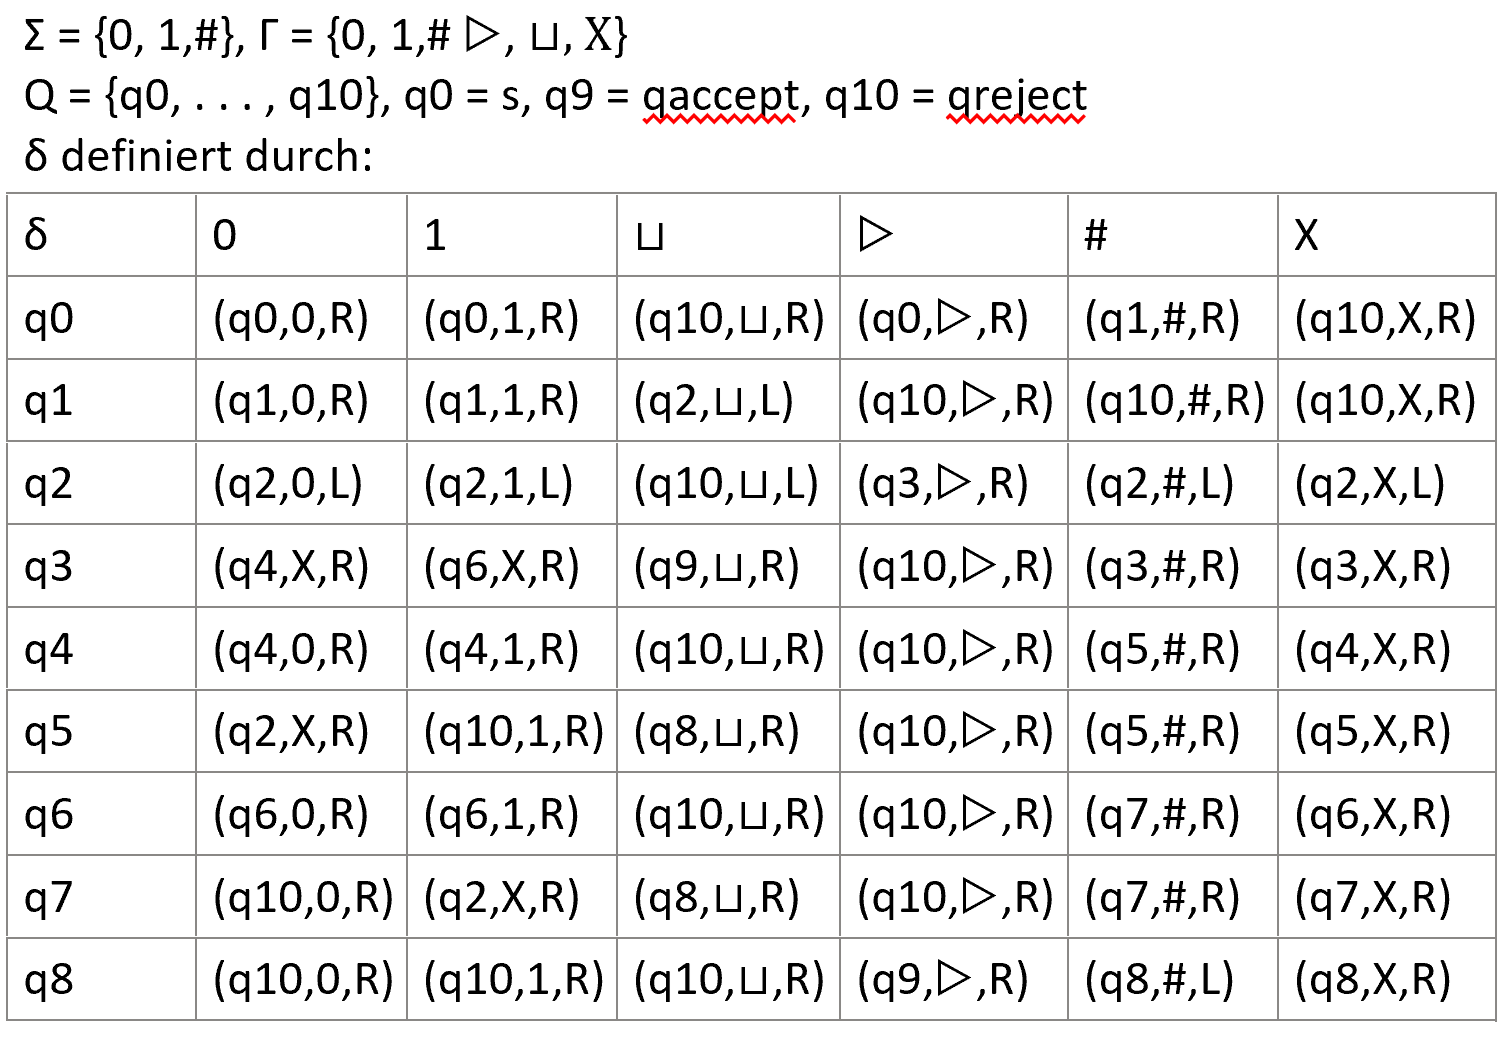
\includegraphics[scale=0.3]{image.png}
  }
\end{exercise}

\begin{exercise}[6]{Rekursive Aufzählbarkeit}
  Zeigen Sie, dass folgende Sprache rekursiv aufzählbar ist.
  \[ L = \left\{(\langle M\rangle, w ,d)\middle| \begin{array}{c} d\in\mathbb{N}\mbox{ und }M\mbox{ akzeptiert die Eingabe }w\\ \mbox{und benötigt dafür mindestens }d\mbox{ Schritte.} \end{array}\right\} \ . \]
  \answer{
    Sei $\tilde{M}$ eine DTM.
    Annahme: Es ist möglich x und d bei einer korrekten Eingabe zu Unterscheiden\\
    $\tilde{M}$ bei Eingabe w $\in \{0,1\}*$ \\

    \begin{enumerate}
      \item \label{aufg4:1} Falls w nicht der Form $\langle M\rangle wd$ ist lehne ab.
      \item \label{aufg4:2} Schreibe auf ein weiteres Band einen Counter, nachdem Model aus Präsenzübung 1.2. mit p=d mit d in Binär.
            Falls dieser auf Null fällt, so wird bei weiteren Abzügen nicht mehr veringert und auf Null gehalten.
      \item \label{aufg4:3} Füge für jeden Zustand $q_i \in Q$ von M einen weiteren Zustand $q_{i+}$ ein, welcher bei Aufruf der Übergangsfunktion (mit $q_i$ in der Eingabe) den Counter um Eins verringert.
            Sei $M'$ diese modifizierte Turingmaschine.
      \item \label{aufg4:4} Simuliere M' mit x
      \item \label{aufg4:5} Wird in 4. festgestellt, dass M' die Eingabe akzeptiert und Counter = 0, akzeptiere $\langle M\rangle wd$.
    \end{enumerate}

    Schritt \ref{aufg4:1} ist möglich, da Gödelnummer eindeutig sind, $w$ und $d$ unterschieden werden können (nach Annahme).\\
    Schritt \ref{aufg4:2} ist nach Präsenzübung 1 berechenbar. \\
    Schritt \ref{aufg4:3} kann durch eine Manipulation der Gödelnummer von $\langle M\rangle$ durchgeführt werden,
    da die Zustandsmenge abzählbar ist, gibt es eine endliche Anzahl von Zuständen und damit eine endliche Anzahl
    von Schritten um die veränderte Turingmaschine zu konstruieren. \\
    Ändere $(q_i,X) \rightarrow (q_k,X,D)$ zu $(q_i,X) \rightarrow (q_{i+|Q|},X_H,N)$, $(q_{i+|Q|},X) \rightarrow (q_k,X,D)$ mit X eine beliebige Eingabe und $X_H$ eine Eingabe,
    welche den Bandinhalt nicht ändert. \\
    Schritt \ref{aufg4:4} und \ref{aufg4:5} können durch eine Universelle Turingmaschine berechnet werden. \\

    Nun ist nur noch Z.z, dass $\tilde{M}$ die Sprache L akzeptiert. \\
    Dazu sei die Eingabe $x=\langle M\rangle wd$, da sie sonst nach \ref{aufg4:1} bereits ablehnen würde. Also ist noch Folgendes Z.Z. \\
    \begin{enumerate}[label=\roman*)]
      \item \label{aufg4:i} Falls M die Eingabe x akzeptiert, so akzeptiert $\tilde{M}$ die Eingabe x.
      \item \label{aufg4:ii} Falls M die Eingabe x nicht akzeptiert, so akzeptiert $\tilde{M}$ die Eingabe x nicht.
    \end{enumerate}

    zu \ref{aufg4:i} Ist x $\in$ L, so akzeptiert M und es gab mindestens d übergänge. Folglich wird in der Simulation in Schritt 4 x akzeptiert. Da x $\in$ L gab es mindestens d Übergänge und der Counter ist auf 0. Also wird x nach Schritt 5 akzeptiert. \\

    zu \ref{aufg4:ii} Ist x $\notin$ L, so:
    \begin{enumerate}[label=\alph*)]
      \item \label{aufg4:a} $M$ lehnt $x$ ab.
      \item \label{aufg4:b} $M$ akzeptiert $x$ mit weniger als $d$ Übergängen.
      \item \label{aufg4:c} $M$ kommt bei Eingabe $x$ in eine Endlosschleife.
    \end{enumerate}

    Zu Fall \ref{aufg4:a}: \\
    $\tilde{M}$ würde x auch Schritt 5 nicht akzeptieren. \\
    Zu Fall \ref{aufg4:b}: \\ \\
    Folglich ist der Counter bei dieser Eingabe ungleich Null $\rightarrow$ (Schritt 5) x wird nicht akzeptiert. \\ \\
    Zu Fall \ref{aufg4:c}: \\
    Folglich ist der Counter bei dieder Eingabe Null, aber x wird von M nicht akzeptiert.

    $\rightarrow$ L ist rekusiv abzählbar $\qed$
  }
\end{exercise}

\end{document}
